%%%%%%%%%%%%%%%%%%%%%%%%%%%%%%%%%%%%%%%%%%%%%%%%%%%%%%%%%%%%%%%%%%%%%%%
\documentclass[num-refs]{wiley-article} % Courtesy Overleaf

% Add additional packages here if required
\usepackage[numbers]{natbib}
\usepackage{natmove}
\usepackage{setspace}

%\changefontsizes{10pt}
\raggedbottom


% Update article type if known
\papertype{Original Article}
\paperfield{}

%\abbrevs{%
%         ABC, a black cat;
%	     DEF, doesn't ever fret;
%	     GHI, goes home immediately.
%     }

\title{Estimation for iron contamination in Si solar cell by ideality factor: deep neural network approach}

\author[1]{Oleg~Olikh}
\author[1]{Oleg~Lozitsky}
\author[1]{Oleksii~Zavhorodnii}

%\author[1\authfn{1}]{Oleg~Olikh}
%\author[1\authfn{1}]{Oleg~Lozitsky}
%\author[1\authfn{2}]{Oleksii~Zavhorodnii}


%\contrib[\authfn{1}]{Equally contributing authors.}

\affil[1]{Taras Shevchenko National University of Kyiv, 64/13, Volodymyrska Street, Kyiv, 01601, Ukraine}
%\affil[2]{Department, Institution, City, State or Province, Postal Code, Country}

\corraddress{Olikh O, Taras Shevchenko National University of Kyiv, 64/13, Volodymyrska Street, Kyiv, 01601, Ukraine}
\corremail{olegolikh@knu.ua}

%\presentadd[\authfn{2}]{Department, Institution, City, State or Province, Postal Code, Country}

\fundinginfo{National Research Foundation  of Ukraine, Project Number: 2020.02/0036}

%\runningauthor{F. Author et al.}

\begin{document}


Dear editor,

We like to express our appreciation to the reviewers for their comments.
We are resubmitting the revised version of the paper number PIP--21--281.
We have studied the comments of the reviewer carefully, and have changed the text according to the comments they
have listed.
%The location of revisions is pointed by blue color in ``MarkedManuscript.pdf''.
Below we refer to each of the reviewer’s comments.

\subsection*{Response to Reviewer \#1 }



\noindent
\textcolor[rgb]{0.00,0.50,1.00}{\textbf{Comment~1.}}
\emph{A solar cell with BSF is chosen as the basis of the work, claiming that
"BSF is one of the popular designs used for industrial mass production...",
but this is no longer the case, BSF solar cells are present in the market due to old manufacturing lines that are still operative, but the standard now is PERC technology.
If the training of the network is based on SCAPS simulations, why was not trained with a PERC structure?
At least, some hint on how results would be with a PERC structure should be given.
(By the way, the BSF in this work is made with B-doping, which is also a minoritary approach at the industrial level, where BSF is of Aluminium).}

\vspace{0.5cm}
\noindent
\textcolor[rgb]{0.51,0.00,0.00}{\textbf{Reply:}}
The Reviewer is absolutely right and PERC technology will be dominant in close future.
But now the part of BSF solar cells is still big enough --- see Fig.~\ref{fig_BSF}.
%\cite{GreenRew2019,WilsonRew2020}


\begin{figure}[b]
\centering
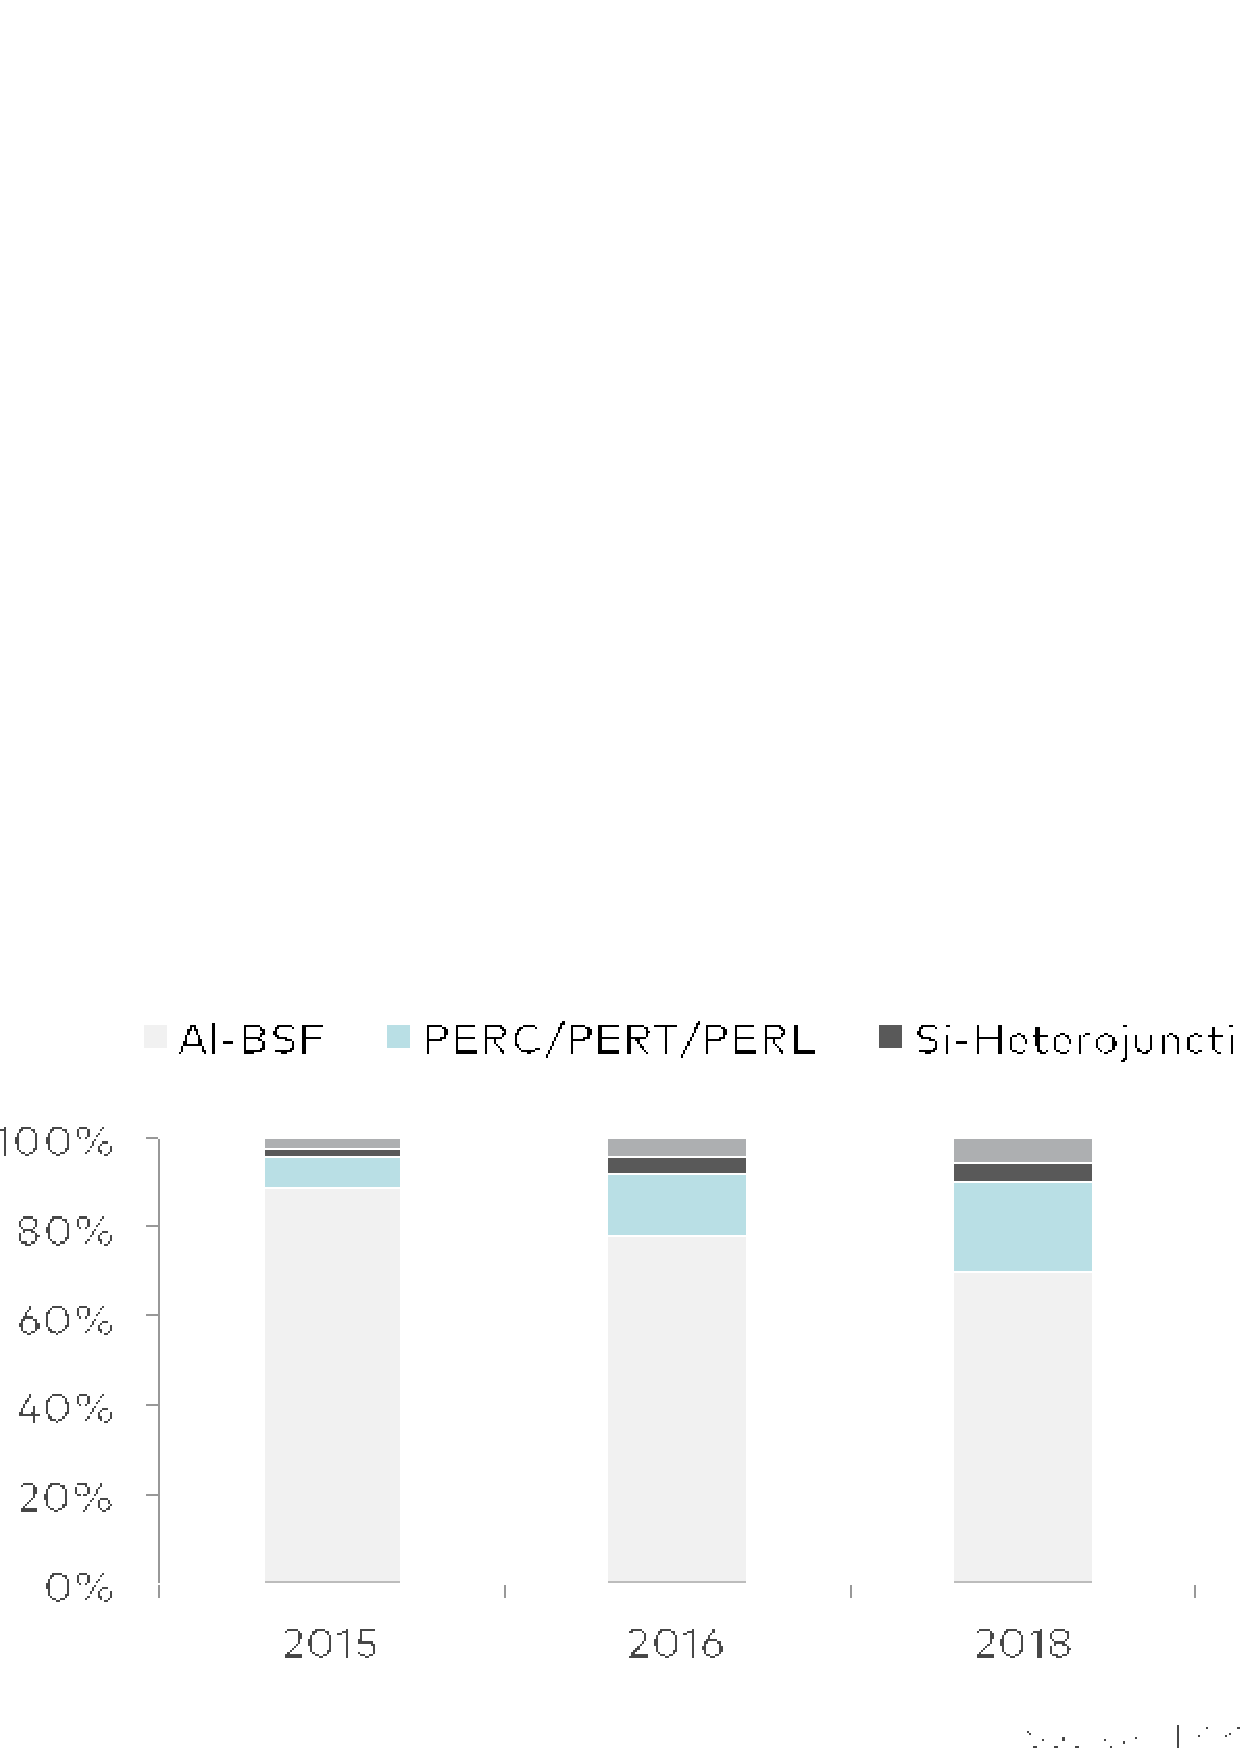
\includegraphics[width=0.48\textwidth]{BSF_PERC1}
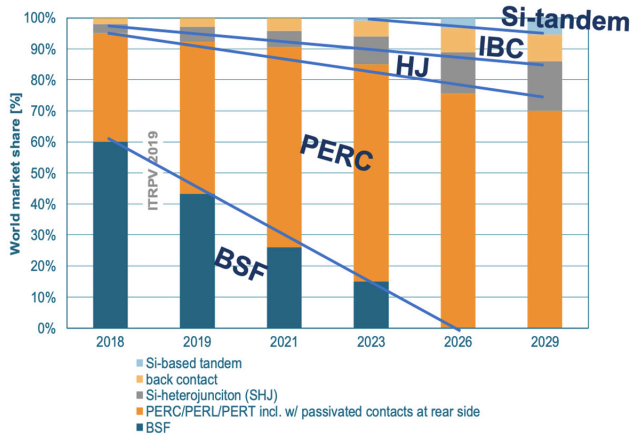
\includegraphics[width=0.48\textwidth]{BSF_PERC2}
\caption{Projected manufacturing capacity share of different
silicon--based cell technologies.
Sources:  https://www.aleo-solar.com/perc-cell-technology-explained/
(left panel), \cite{GreenRew2019} (right panel).
}
\label{fig_BSF}
\end{figure}

SCAPS-1D is a one-dimensional solar cell simulation programme and
the modeling of PERC solar cells with rear contact, which is
inhomogeneous, in surface is hard task.
We understand the limitations of 1D simulators and noted about this in the Conclusion.

We agree that it would be better to use Al-doped $p^+$-layer, but please consider the following.
The simulated IV curves were used to obtain the ideality factor value $n$.
According used two-diode model,
$n$ characterizes current of second (so-called recombination)  diode;
the current of second diode current is due to recombination within
the depletion region mainly \citep{Breitenstein2013}.
The $p^+$--layer influence on mentioned process is rather determined by
pulling electric field.
Therefore the kind of doping atom in $p^+$--layer is not very important for our simulation.
In the case of $n^+-p-p^+$ structure with Al-doped base the new training data set is needed,
but the proposed deep-learning oriented approach to determining the impurity concentration remains valid.
On the other hand, the recombination in the rear surface region is not dominant
in $n$ value determination.
In our opinion, the trained DNN can be applied to PERC solar cell in wich
i)~the base is boron-doped;
ii)~the iron-related deep levels are the main reason of defect-assisted recombination.


The text was revised and the some information (hint) was added in page


\vspace{1cm}
\noindent
\textcolor[rgb]{0.00,0.50,1.00}{\textbf{Comment~2.}}
\emph{As far as I understand, the simulation with SCAPS could be improved: emitter and BSF are uniform and this is not the case in reality.
There is no mention to the metallization, are there no contacts?
There should be, and they will influence the carrier transport and also the surface recombination velocities in the metal-semiconductor interface, among others.}

\vspace{0.5cm}
\noindent
\textcolor[rgb]{0.51,0.00,0.00}{\textbf{Reply:}}
The flat bands conditions were assumed for metal contacts on on the rear and
front surfaces.
A sentence was added in text. 
Let us note that it is common practice not to pay special attention in SCAPS simulation 
to contacts in the case of
the barrier absence --- e.g., see \cite{SCAPSuseSi4,SCAPSuseSi1,SCAPSuse1,SCAPSuse5,ScapsUse10}.



The Reviewer is correct about the way of SCAPS simulation improvement.
In the present paper, we have concentrated on recombination in the SC base region,
which mainly determine ideality factor value.
The non-uniformities of emitter and  BSF-layer affect much weaker on $n$ value.
But the Reviewer’s suggestion is very interesting, and must be done in the 
future. 

\vspace{1cm}
\noindent
\textcolor[rgb]{0.00,0.50,1.00}{\textbf{Comment~3.}}
\emph{Why a voltage sweep restricted to 0.45 V?
This is rather low when compared to the voltages at the maximum power point of BSF solar cells...
Wouldn't it influence in the extraction of the ideality factor values?}

\vspace{0.5cm}
\noindent
\textcolor[rgb]{0.51,0.00,0.00}{\textbf{Reply:}}
We used the two-diode model to fit the simulated data.
According to the two-diode model, the dark SC current is given by
\begin{equation}
\label{eqIVd}
    I=I_{01}\left[\exp\left(-\frac{q(V-R_sI)}{kT}\right)-1\right]
      + I_{02}\left[\exp\left(-\frac{q(V-R_sI)}{nkT}\right)-1\right]
      +\frac{V-R_sI}{R_{sh}}\,,
\end{equation}
where
$I_{01}$ and $I_{02}$ are the saturation currents,
$R_{sh}$ and $R_s$ are the shunt and series resistances.
The two-diode model is often applied for description of real Si SCs
and the first diode represents the ``ideal'' diode and
first term in Eq.~(\ref{eqIVd})
current is due to recombination in the base
and the emitter, including their surfaces;
the second diode is the so-called recombination diode
and second term is due to recombination within
the depletion region \citep{Breitenstein2013}.

The typical IV curves are shown in Fig.~\ref{fig_IV}.
It is seen that the contribution of recombination diode current is essential at low bias only.
At $V\simeq 0.25$~V the first term in Eq.~(\ref{eqIVd}) is
by an order of magnitude larger than the second term.
Similar situation is observed for
experimental IV curves --- see Fig.~9 in Manuscript.
The ideality factor value is related to slope of recombination current
dependence on voltage in semi-logarithmic scale.
Therefore the voltage range $(0-0.45)$~V is quite sufficient for an accurate determination of the ideality factor values.

\begin{figure}[t]
\centering
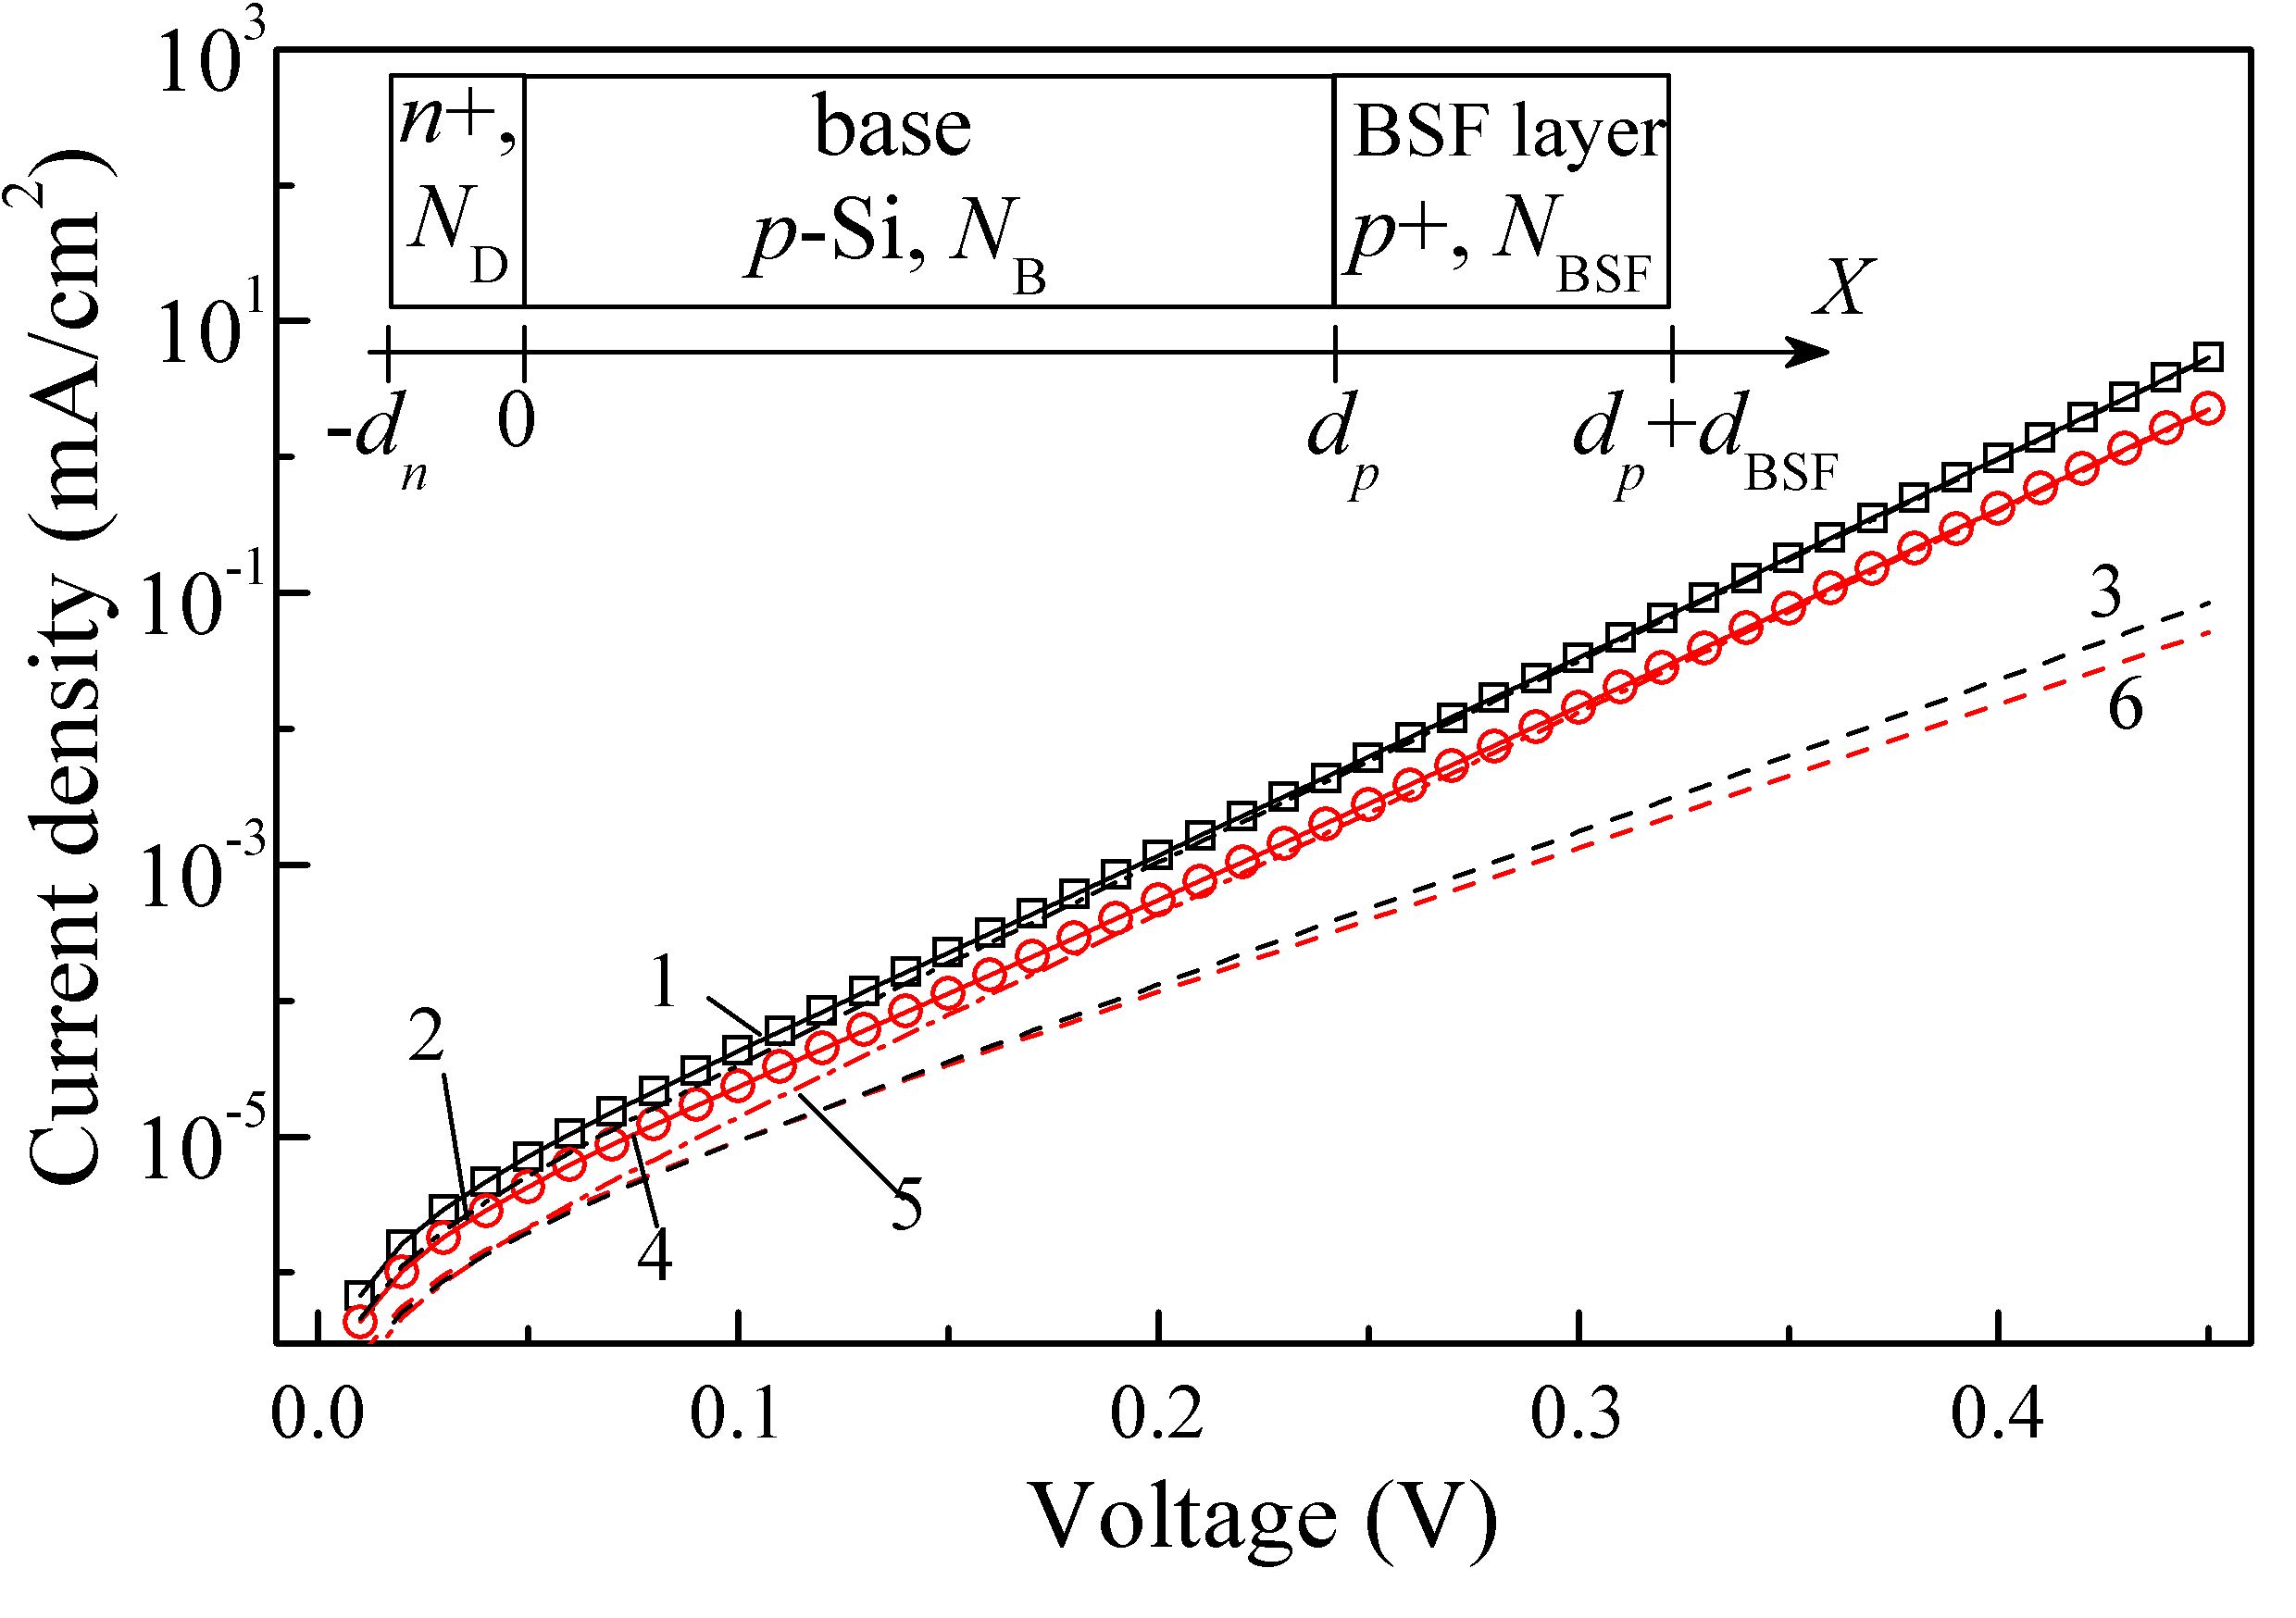
\includegraphics[width=0.5\textwidth]{FigIV}
\caption{Simulated IV characteristic (marks)
and its fitting by Eq.~(\ref{eqIVd}) (solid lines 1 and 4).
The dashed (3, 6) and dotted--dashed (2, 5)
lines represent the recombination diode currents and the ``ideal'' diode currents, respectively.
$N_\mathrm{B} = 10^{17}$~cm$^{-3}$, $N_\mathrm{Fe} = 10^{13}$~cm$^{-3}$,
$T = 340$~K, $d_p = 180$~$\mu$m.
The results for Fe-case (circles, curves 4-6, red)
and Fe-FeB case (squares, curves 1-3, black) are presented.
Inset: Structures, which are used in the simulation.
}
\label{fig_IV}
\end{figure}

The information was added in page


\vspace{1cm}
\noindent
\textcolor[rgb]{0.00,0.50,1.00}{\textbf{Comment~4.}}
\emph{I am not sure that I interpret well the results in table 5.
In the text the authors state that "the results even exceed expectations".
But what I see is that the predictions fail in general, largely for the trained dataset cases, but also for the full dataset.
There is some discussion on why DNN$_{FeFeB-Fe}$ performs worse than DNN$_{FeFeB}$ and that is Ok... but DNN$_{FeFeB}$ also fails in many cases, isn't it?
(temperatures higher than 300K for the higher Fe content, 100\% or more error for the training dataset...).
}

\vspace{0.5cm}
\noindent
\textcolor[rgb]{0.51,0.00,0.00}{\textbf{Reply:}}
The text was revised.

\vspace{1cm}
\noindent
\textcolor[rgb]{0.00,0.50,1.00}{\textbf{Comment~5.}}
\emph{In the jargon, we do not talk of surface resistance, but sheet resistance.
Also, it is the first time that I read the "anti-recombination isotype barrier" for a high-low junction or a BSF.}

\vspace{0.5cm}
\noindent
\textcolor[rgb]{0.51,0.00,0.00}{\textbf{Reply:}}
The Reviewer is absolutely right.
We have revised the text accordingly. 

\vspace{1cm}
\noindent
\textcolor[rgb]{0.00,0.50,1.00}{\textbf{Comment~6.}}
\emph{It is mentioned in the paper that there is Suplementary Material, but I have not had the opportunity to read it.}

\vspace{0.5cm}
\noindent
\textcolor[rgb]{0.51,0.00,0.00}{\textbf{Reply:}}
We apologize for embarrassing.
But we are in confusion:
Reviewer \#2 mentioned about the data in the table of Supplementary Material.


\vspace{1cm}
\noindent
\textcolor[rgb]{0.00,0.50,1.00}{\textbf{Comment~7.}}
\emph{On the other hand, the paper needs a thorough revision of English, preferably by a native or bilingual speaker.
English is not my mother tongue, but I think that there are many expressions that are not correct, and make the reading difficult.
From the abstract ("The low-cost and express...", "an ideality factor values"...)
to the conclusions ("not numerous input parameters can be multiplied and transformed to the picture and apply a vision model..."(?),
and a lot in between: "both for microelectronics, logic technologies and solar cells",
"the various semiconductor barrier structures", "practical using", "Fours", "SFB", "in our further calculation",
"simulated with using", "in comparing with", "more narrow", etc. etc. }

\vspace{0.5cm}
\noindent
\textcolor[rgb]{0.51,0.00,0.00}{\textbf{Reply:}}
We are sorry for English.
The text was revised by bilingual speaker and we hope for language improving.




\subsection*{Response to Reviewer \#2 }


\textcolor[rgb]{0.00,0.50,1.00}{\textbf{Comment~1.}}
\emph{2 Simulation details}

\emph{It is assumed that all SRH recombination in the device come from iron impurities and the associated deep level defects.
It seems necessary to discuss its validity, and it could be interesting to put it against the fact that Al-BSF devices based on Czochralski silicon wafers are considered.
More generally, if another type of defects is present in the solar cell, also inducing SRH recombination,
is it possible to estimate to what extend are the DNNs trained here still accurate ? }

\vspace{0.5cm}
\noindent
\textcolor[rgb]{0.51,0.00,0.00}{\textbf{Reply:}}
The text was revised.


\vspace{1cm}
\noindent
\textcolor[rgb]{0.00,0.50,1.00}{\textbf{Comment~2.}}
\emph{When Fe-FeB and Fe cases are presented, it could be clearer to provide very few more explanations on both types of defects,
and the important fact that iron-boron pairs can be temporarily dissociated, providing the Fe case,
through the heat treatment or high illumination already mentioned. }

\vspace{0.5cm}
\noindent
\textcolor[rgb]{0.51,0.00,0.00}{\textbf{Reply:}}
The corresponding corrections were done in page


\vspace{1cm}
\noindent
\textcolor[rgb]{0.00,0.50,1.00}{\textbf{Comment~3.}}
\emph{3 Deep neural network models}

\emph{
It is clear how the main training dataset is created, and how the 4 * 9 * 11 * 19 = 7524 IV curves are generated.
However, the definition of the test datasets and the values for temperature,
base thickness, iron concentration and doping level are not clear for each T-varied, d-varied, etc. test set. }

\vspace{0.5cm}
\noindent
\textcolor[rgb]{0.51,0.00,0.00}{\textbf{Reply:}}
The sample of values which used for Fe-varied dataset was added in page  





\vspace{1cm}
\noindent
\textcolor[rgb]{0.00,0.50,1.00}{\textbf{Comment~4.}}
\emph{
For instance, in the case of the T-varied test set, it is mentioned that the same base thickness,
iron concentration and doping level values are used as in training dataset.
However, 4 * 9 * 19 = 684 and the amount of 894 IVs can’t be explained by multiplying with any number of temperature values.
In Supplementary Material, the associated summary table do neither explain this value 894. More generally these tables are difficult to interpret. It is possible that the subset of 144 values for T-varied test has been duplicated. }

\vspace{0.5cm}
\noindent
\textcolor[rgb]{0.51,0.00,0.00}{\textbf{Reply:}}
The Reviewer is absolutely right:
i)~the subset of 144 values for T-varied test dataset has been duplicated;
ii)~Table in Supplementary Material has a mistakes and is not clear.
The correct values of $d_p$, $N_\mathrm{B}$, and $N_{\mathrm{Fe}}$ were listed in Table,
but we have a some problems with addition and multiplication.
We apologize for the inattention.
Table in Supplementary Material was revised.

\vspace{1cm}
\noindent
\textcolor[rgb]{0.00,0.50,1.00}{\textbf{Comment~5.}}
\emph{4 Results and discussion}

\emph{
On figures 4, 5, 6 and 7, very interesting results are presented, and analyses of the dependence of estimation
error with temperature, boron or iron densities and base thickness are well done.
However, it seems that the same error statistics of results obtained on test datasets
(instead of training dataset) would more directly assess the quality of predictions by the DNNs.
For instance, the Fe-varied dataset has been identified to be
the closest to “real demand” or results obtained with the all-varied dataset would also be most probably very useful.
Such results could be showed in Supplementary Material, in the same form as figures 4, 5, 6 and 7. }

\vspace{0.5cm}
\noindent
\textcolor[rgb]{0.51,0.00,0.00}{\textbf{Reply:}}
The text was revised.



%\noindent
%\textcolor[rgb]{0.00,0.50,1.00}{\textbf{Comment~1.}}
%\emph{In Fig. 4, the numbers identifying the different curves are missing.}
%
%\noindent
%\textcolor[rgb]{0.51,0.00,0.00}{\textbf{Reply:}}
%The curves' numbers were added.
%We apologize for the inattention.
%
%
%\vspace{1cm}
%\noindent
%\textcolor[rgb]{0.00,0.50,1.00}{\textbf{Comment~2.}}
%\emph{Figure 6 is not so relevant, and could be given as supplementary information}
%
%\noindent
%\textcolor[rgb]{0.51,0.00,0.00}{\textbf{Reply:}}
%Figure~6 was transferred to the Supplementary material,
%the text was revised (page~5, column~1, paragraph~2).
%
%
%\subsection*{Response to Reviewer \#3 }
%
%\noindent
%\textcolor[rgb]{0.00,0.50,1.00}{\textbf{Comment~1.}}
%\emph{Page 1, column 2, line 1: The lattice deformation amplitude should have a unit.}
%
%\noindent
%\textcolor[rgb]{0.51,0.00,0.00}{\textbf{Reply:}}
%The ``relative deformation'' was meant.
%The term ``strain'' is used in the revised version.
%
%
%\vspace{1cm}
%\noindent
%\textcolor[rgb]{0.00,0.50,1.00}{\textbf{Comment~2.}}
%\emph{Page 1, column 2, paragraph 3: The origin of the iron in the diodes should be explained. How are the diodes contaminated with iron? }
%
%\noindent
%\textcolor[rgb]{0.51,0.00,0.00}{\textbf{Reply:}}
%The technological process of solar cells (SCs) manufacturing from Cz-p-Si wafers included the formation of separating and isotype barriers ($n^+$-$p$ and $p$-$p^+$ junctions) by diffusion of phosphorus (POCl$_3$) and boron (BCl$_3$) from the gas phase, respectively; thermal oxidation; thermal annealing; photolithography; etching the dividing groove; chemical treatments; magnetron sputtering of aluminum contacts to the front and back sides.
%
%It has been found that some SC lots have significantly worse parameters compared to typical solar cells for this technological process.
%In particular, the photoconversion efficiency was almost halved.
%The analysis showed that the reason for such a deterioration in the SC parameters is a sharp drop in the diffusion length of minority charge carriers (electrons) $L_n$ in the SC base.
%Additional experiments with thermal annealing at temperatures of 200$^\circ$C and 90$^\circ$C
%(the procedure is described by Tayyib~\emph{et al.}\cite{TAYYIB201221})
%showed that the decrease in $L_n$ value is caused by iron impurities available in the SC base at concentrations up to $4\cdot10^{13}$~cm$^{-3}$.
%It has also been found that the source of iron impurity is insufficiently pure chemicals that were used for chemical treatments in the technological process, obtained from another supplier.
%These reagents were the source of contamination in the process of manufacturing experimental SC samples.
%
%To study the effect of ultrasonic loading on the kinetics of the transformation  of iron-boron pairs, samples with varying degrees of iron contamination (iron concentration $2\cdot10^{12}$-$4\cdot10^{13}$~cm$^{-3}$) were taken.
%
%More detailed information about iron sources was added (page~1, column~2, paragraphs~3 and 4).
%
%
%\vspace{1cm}
%\noindent
%\textcolor[rgb]{0.00,0.50,1.00}{\textbf{Comment~3.}}
%\emph{Page 1, column 2, paragraph 5: How was the excess carrier density, which is induced by the LED illumination, estimated? This point should be explained. }
%
%\noindent
%\textcolor[rgb]{0.51,0.00,0.00}{\textbf{Reply:}}
%The excess carrier density was estimated by using open-circuit voltage value $V_\mathrm{OC}$.
%According to Sachenko \emph{et. al.}\cite{JAPSach}
%\begin{equation}
%  \Delta n=-\frac{n_0}{2}+\sqrt{\frac{n_0^2}{4}+n_i\exp\left(\frac{qV_\mathrm{OC}}{kT}\right)}
%\end{equation}
%where
%$n_0$ is the equilibrium electron concentration,
%$n_i$ is the intrinsic electron concentration.
%
%The short information was added to the revised manuscript (page~2, column~1, paragraph~3).
%
%
%\vspace{1cm}
%\noindent
%\textcolor[rgb]{0.00,0.50,1.00}{\textbf{Comment~4.}}
%\emph{Figure 2: Short circuit current has the unit $\mu$A not $\mu$m.}
%
%\noindent
%\textcolor[rgb]{0.51,0.00,0.00}{\textbf{Reply:}}
%The reviewer is quite right.
%The graph was corrected.
%
%
%\vspace{1cm}
%\noindent
%\textcolor[rgb]{0.00,0.50,1.00}{\textbf{Comment~5.}}
%\emph{Page 2, column 2, paragraph 1: The materials doping level is given on page 1 with 10 Ohm cm. This is about 1.4e15cm$^{-3}$ and not 1.4e16cm$^{-3}$ as stated here.}
%
%\noindent
%\textcolor[rgb]{0.51,0.00,0.00}{\textbf{Reply:}}
%The reviewer is quite right.
%It was a slip.
%The correction is done.
%
%
%\vspace{1cm}
%\noindent
%\textcolor[rgb]{0.00,0.50,1.00}{\textbf{Comment~6.}}
%\emph{Equation 7: The unit of the pre-factor is missing. }
%
%\noindent
%\textcolor[rgb]{0.51,0.00,0.00}{\textbf{Reply:}}
%The Equation was corrected.
%
%\vspace{1cm}
%\noindent
%\textcolor[rgb]{0.00,0.50,1.00}{\textbf{Comment~7.}}
%\emph{Page 3, column 1, paragraph 3: The obtained iron concentration is compared to results obtained from diffusion length measurements. There should be a reference to these measurements or more details should be given.}
%
%\noindent
%\textcolor[rgb]{0.51,0.00,0.00}{\textbf{Reply:}}
%The diffusion length before ($L_{n0}$) and after ($L_{n1}$) pair dissociation was measured using spectral dependencies of short circuit current\cite{LnIscMethod}.
%Then the iron concentration was determined by using Zoth and Bergholz\cite{FeB_Zong} equation:
%\begin{equation}
%  N_\mathrm{Fe}(\mathrm{cm}^{-3})=1.06\cdot10^{16}\left(\frac{1}{L_{n1}^2}-\frac{1}{L_{n0}^2}\right)(\mu\mathrm{m}^{-2})
%\end{equation}
%
%The short information was added to the revised manuscript.
%
%\vspace{1cm}
%\noindent
%\textcolor[rgb]{0.00,0.50,1.00}{\textbf{Comment~8.}}
%\emph{Figure 4: The numbers of the curves given in the caption are not included in the graphs. This must be improved otherwise the figures cannot be understood. Each graph should also be marked by a letter. What is ``G'' at the x-axis of the inset? This should be explained. }
%
%
%\noindent
%\textcolor[rgb]{0.51,0.00,0.00}{\textbf{Reply:}}
%The graphs were revised.
%The curves' numbers were added.
%Each graph was marked by a letter.
%``G'' was changed by ``Will'' (radiation intensity of halogen lamp).
%We apologize for the inattention.
%
%
%\vspace{1cm}
%\noindent
%\textcolor[rgb]{0.00,0.50,1.00}{\textbf{Comment~9.}}
%\emph{Figure 5: This plot is confusing and must be revised. What is the main statement of this figure? What are the differences between the samples and why do the results change from sample to sample? The axes should have the same scaling. What are the light blue bars in (a)? }
%
%\noindent
%\textcolor[rgb]{0.51,0.00,0.00}{\textbf{Reply:}}
%Figure~5 was changed by Table~I.
%The main assignment of this data is an illustration of
%
%\noindent
%i)~USL actually does not influence the $\tau_\mathrm{dis}$  magnitude;
%
%\noindent
%ii)~some pairs do not dissociate under illumination in the USL case when light--induced pair dissociation is close to saturation.
%The decrease in illumination intensity reduces the last effect at the given illumination times.
%
%The main differences between the samples are the iron concentrations.
%However, data show that
%the effect of ultrasound does not qualitatively change with the iron concentration alteration
%(from sample to sample).
%The value of acousto-induced change in $N_\mathrm{Fe,fit}$ value depends on ultrasound intensity
%(see data for sample SC350-1, $W_\mathrm{ill}=0.16$~W/cm$^2$) and frequency.
%
%
%The dissociation rate of FeB pairs depends on iron concentration, light intensity, and
%temperature\cite{Schmidt2019,FeBLight2,FeBKin2019,Lagowskii1993}.
%There is a reason of $\tau_\mathrm{dis}$ value change from panel to panel in Fig.~5 in the unrevised manuscript (from row to row in Table~I in the revised manuscript)
%
%The light blue bars in Fig.~5(a) (the unrevised manuscript) corresponded to another ultrasound intensity
%(0.6~W/cm$^2$).
%
%\vspace{1cm}
%\noindent
%\textcolor[rgb]{0.00,0.50,1.00}{\textbf{Comment~10.}}
%\emph{Main Problem}
%\emph{The impact of ultrasound on the iron-boron-pair reaction was first reported by Ostapenko and Bell in 1995 [1]. They found that the iron boron pairs dissociate due to an ultrasound treatment. This is in contradiction to the findings, which are reported herein. In the contribution under review it is found that the association of the FeB pairs is enhanced by the ultrasound treatment. This contradiction must absolutely be discussed by the authors otherwise the manuscript cannot be published.}
%
%\emph{
%[1] S. S. Ostapenko and R. E. Bell, "Ultrasound stimulated dissociation of Fe-B pairs in silicon," J. Appl. Phys., vol. 77, no. 10, p. 5458, 1995.
% }
%
%\noindent
%\textcolor[rgb]{0.51,0.00,0.00}{\textbf{Reply:}}
%We do not keep silent about reports Ostapenko \emph{et al.} --- see Refs.26,27;
%page~3, column~2, paragraph~1; page~7, column~2, paragraph~1 in the unrevised manuscript.
%But Reviewer is right and more attention should be paid to the comparison of the findings.
%
%In our opinion,
%the reported herein and previous results have a lot in common.
%According to Ostapenko \emph{et al.}\cite{Ostapenko1995SST}
%Fe$_i$ has to ``jump'' to the next nearest interstitial under ultrasound action;
%we state about the decrease in Fe$_i$ migration energy value
%as well as enhance of Fe$_i$ diffusivity
%in case of ultrasound loading.
%The effectiveness of ultrasound influence increase with the rise of temperature in both cases:
%according to Ostapenko \emph{et al.},\cite{Ostapenko1994APL,Ostapenko1995SST}
%the diffusion length increases from 10.5~$\mu$m to 13~$\mu$m at 20$^\circ$C and up to
%22~$\mu$m at 70$^\circ$C;
%$\Delta E_\mathrm{US}$ increases from 3~meV to 8~meV with temperature change
%from 300~K to 340~K at  $f_\mathrm{US}=0.3$~MHz and $W_\mathrm{US}=0.76$~W/cm$^2$
%(Fig.6 in the revised manuscript).
%The difference in the action of ultrasound
%(the iron-boron pairs dissociation or the enhancing of pairing)
%is associated with the difference in the intensity of the acoustic influence.
%For instance, the researchers used acoustic strain $\xi_\mathrm{US}=10^{-5}$-$10^{-4}$
%was used\cite{Ostapenko1995}
%to dissociate FeB pairs in Cz--Si.
%Furthermore,
%Ostapenko and Bell\cite{Ostapenko1995} regarded the resonance condition of
%pair reorientation (first step of dissociation) and used $25-70$~kHz.
%In our case,  $\xi_\mathrm{US}<2\cdot10^{-6}$ and $f_\mathrm{US}=2-30$~MHz are deficient to effectively overcome the Coulombic attraction between Fe$_i^+$ and B$_s^-$.
%Additionally, the presented data show that the effectiveness of acoustically--induced change
%decreases as the ultrasound frequency increases.
%
%It should be noted that Ostapenko \emph{et al.}\cite{Ostapenko1994APL} asserted
%``in the  case  of predominant  dissociated  pairs,  it [ultrasound treatment] may promote  the
%pairing reaction'' (page~1557, column~1, paragraph~2).
%In our case, the predominant  dissociation was realized by intense illumination, and then
%the ultrasound loading accelerated pairing.
%Thus, the reported results provided empirical evidence  for the above-mentioned prediction.
%
%
%On the other hand, a certain manifestation of partial acoustically-induced FeB dissociation could be
%a decrease in the concentration of pairs, which dissociate under illumination in the USL case.
%In fact, if some pairs were dissociated by  ultrasound waves, which had been pre-exited
%in the sample with a high initial  fraction of paired Fe,
%they can not be dissociated under illumination.
%The decrease in the temperature   or photon quantity leads to reduce in the set of FeB, which was modified by ultrasound, or in the set of FeB,
%which was modified by the capture of light-induced electrons, respectively.
%Sets cease to overlap and $N_\mathrm{Fe,fit}(W_\mathrm{US}>0)\simeq N_\mathrm{Fe,fit}(W_\mathrm{US}=0)$ --- see Table~I in the revised manuscript.
%
%
%Finally, let's summarize the differences between the manuscript and previously reported results.
%Ostapenko \emph{et al.}\cite{Ostapenko1995,Ostapenko1994APL,Ostapenko1995SST}
%investigated the change in silicon properties (diffusion length) \textbf{after}
%the action of ultrasound with high (above threshold) intensity.
%This is the so-called ultrasound treatment mode of operation
%and results  can be used to develop a new approach to semiconductor properties modification.
%Our manuscript is devoted to the modification of the process
%(short circuit current kinetics or FeB transformation),
%\textbf{during} subthreshold acoustic wave propagation.
%This is ultrasound loading mode,
%which can be used for acoustically controlled tuning of the technological processes.
%
%The additional information was added to the revised manuscript
%(page~7, column~1, last paragraph; page~7, column~2, paragraph~1).





%\bibliographystyle{rss}
\bibliographystyle{WileyNJD-Harvard}
\bibliography{olikh}


\end{document}
